\documentclass[10pt,twocolumn]{article}

\usepackage[a4paper,margin=1.5cm]{geometry}
\usepackage{authblk}
\usepackage{setspace}
\usepackage[compact]{titlesec}
\pdfoptionpdfminorversion=4
\usepackage{graphicx}
\usepackage[separate-uncertainty=true]{siunitx}
\usepackage{hyperref}
\usepackage{amsbsy,amssymb,amsmath,bm}
\usepackage[none]{hyphenat}
\usepackage{float}
\usepackage{booktabs}
\usepackage{xcolor}
\parskip 0.35\baselineskip
\parindent 0mm
\setlength{\textfloatsep}{0.45\baselineskip}
\setlength{\floatsep}{0.35\baselineskip}
\setlength{\intextsep}{0.35\baselineskip}
\renewcommand\refname{\vspace{-\baselineskip}}
\graphicspath{{figures/}{docs/figures/}{figures/Detector_performance_analysis_Rn222_activity_normalized/}{docs/figures/Detector_performance_analysis_Rn222_activity_normalized/}{figures/Simulation_output_signal_inference_metrics/}{docs/figures/Simulation_output_signal_inference_metrics/}}

\makeatletter
\renewcommand{\maketitle}{
\twocolumn[
  \begin{center}
    {\LARGE \@title \par}
    \vspace{0.5em}
    {\normalsize \@author \par}
    \vspace{1em}
  \end{center}
]
}
\makeatother

\title{Gamma detection for source localisation in targeted alpha therapy}

\author{
C. De Sio$^{\text{a}}$,
L. Abu Sabah$^{\text{a}}$,
J. Duan$^{\text{a}}$,
Y. Shi$^{\text{a}}$,
S. Williams$^{\text{a}}$,
J. Velthuis$^{\text{a}}$\\
\vspace{0.3em}
\small $^{\text{a}}$School of Physics, University of Bristol, Bristol, United Kingdom
}

\date{}

\begin{document}

\maketitle

\begin{abstract}
Targeted alpha therapies deliver highly localised dose, but treatment
verification depends on knowing whether the radionuclide source remains near
the intended site after administration.  We simulated an AlphaGlue-like
geometry using Geant4, with a thin radioactive glue layer on a water phantom
surrounded by six photon-detector panels.  Retained, broadly diffused, and
locally displaced source states were compared using 50 repetitions of 10,000
primary decays per configuration.  Baseline-subtracted gamma-hit profiles
distinguished retained, diffused, and localised source distributions.  The
diffusion fraction was reconstructed from residual profile features with
\(R^2=0.9987\) and a mean absolute error of about one percentage point, while
localised-source residuals identified displaced activity with mean position
errors of \(16\)--\(\SI{30}{mm}\) across the tested localised fractions.
These results support decay-chain gamma detection as a candidate observable
for post-treatment monitoring and source-retention verification in targeted
alpha therapy.
\end{abstract}

\section{Introduction}

Targeted alpha therapy is attractive because alpha particles can deliver a
large dose over a short range.  This locality is also a practical challenge:
the delivered dose depends not only on the administered activity, but on
whether the radioactive material and its progeny remain near the target,
diffuse into adjacent tissue, or are transported through biological
processes~\cite{laura,heger}.  The AlphaGlue concept proposes applying
alpha-emitting material to a tumour region in a thin glue layer~\cite{AlphaGlue2025}.
The activity loaded into the glue is known at production, but confirming the
source distribution at treatment time without disturbing delivery remains a
non-trivial verification problem.

This work tests whether gamma emissions from the decay chain can provide a
theranostic monitoring signal.  The study does not model a full clinical
detector response; instead, it asks whether idealised detector-entry patterns
around a phantom contain enough spatial information to distinguish retained,
broadly diffused, and locally displaced source states.  The emphasis is on
baseline-subtracted profiles, because total gamma-hit yield alone is expected
to be a weak localisation observable.

\section{Materials and Methods}

Photon transport was simulated with the Geant4 toolkit~\cite{Geant4}.  The
model places a \(\SI{40}{mm} \times \SI{2}{mm} \times \SI{40}{mm}\)
loaded glue layer on the \(+y\) surface of a
\(\SI{20}{cm} \times \SI{20}{cm} \times \SI{150}{cm}\) water phantom.  Six
photon-detector panels surround the phantom at \(\SI{20}{cm}\) from the
water surface.  Each gamma entry into a detector panel is recorded as one
hit and binned by detector panel and longitudinal position.

\begin{figure}[!tbp]
    \centering
    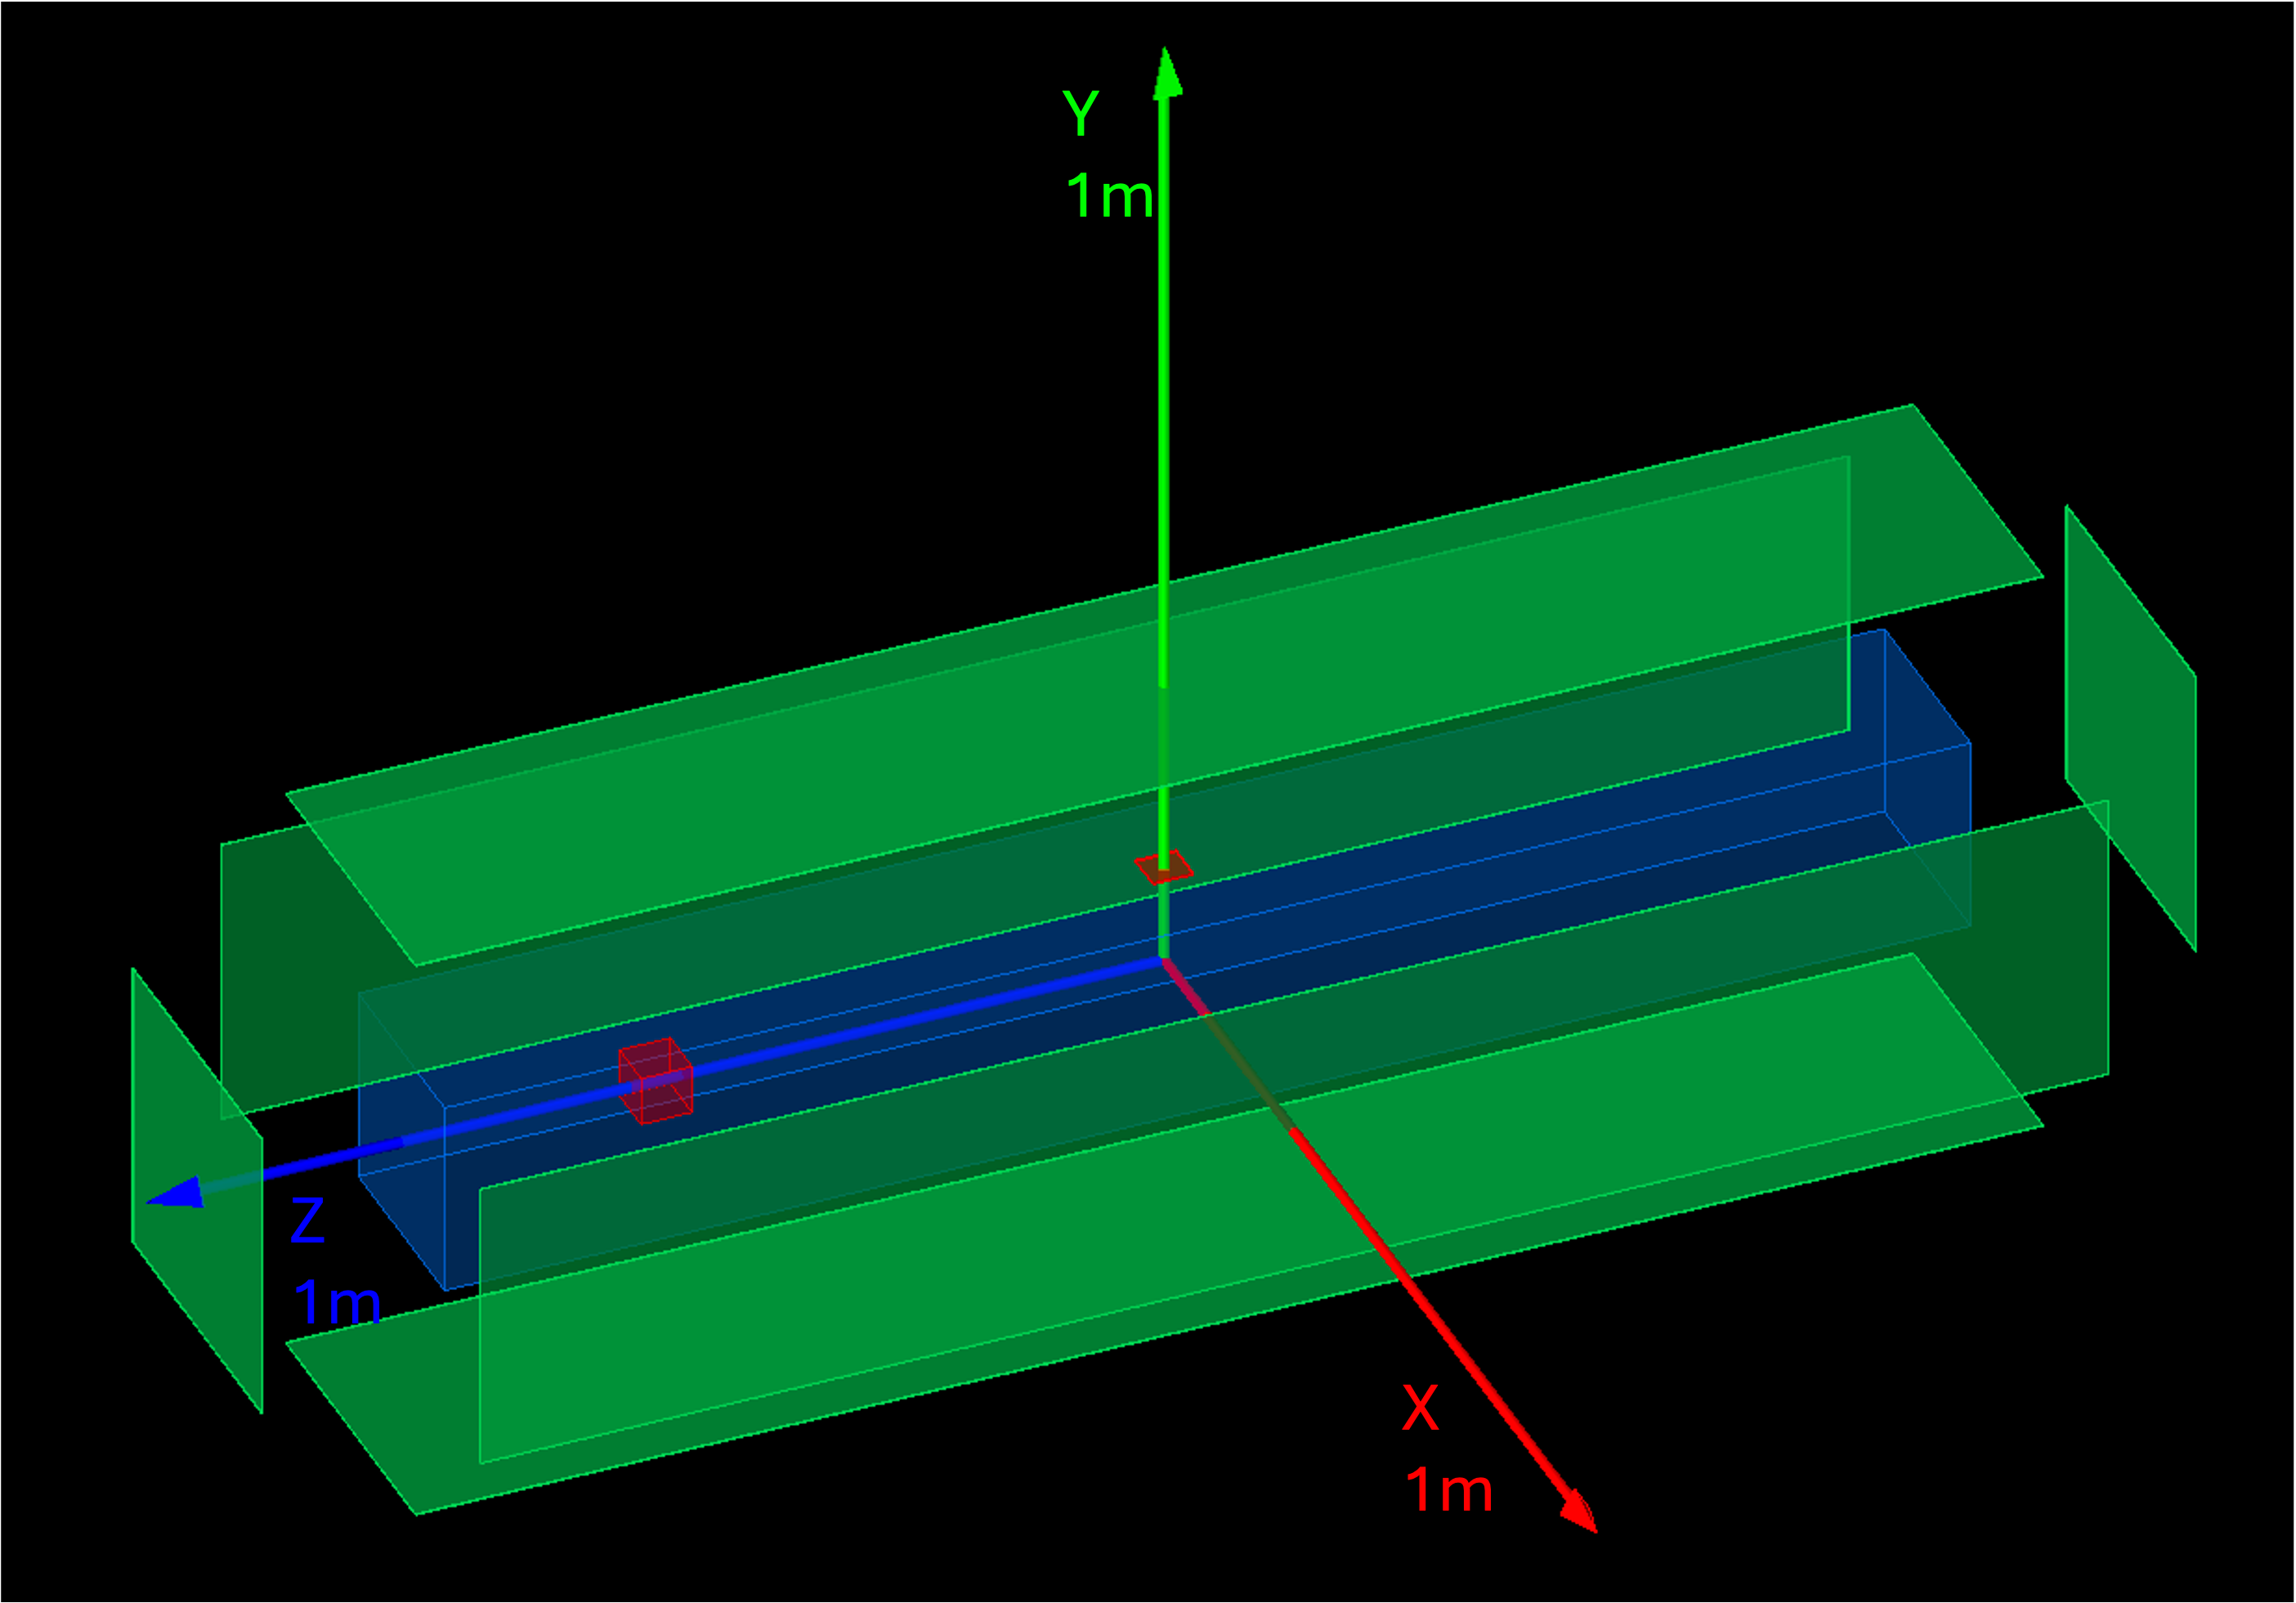
\includegraphics[width=0.72\linewidth]{geometry.png}
    \caption{\textit{Simulation geometry with water phantom, surrounding
    detector panels, and source regions.}}
    \label{fig:geometry}
\end{figure}

Seven source states were studied.  The baseline case places all activity in
the glue layer.  Broad-redistribution cases place 10\%, 50\%, or 90\% of the
activity diffusely in the water volume, with the remaining activity retained
in the glue.  Localised-displacement cases place 20\%, 40\%, or 60\% of the
activity in a compact displaced water region, again with the remainder
retained in the glue.  These source states are sensitivity tests for source
movement rather than patient-specific biological models.

Each source state was simulated with 50 independent repetitions of 10,000
primary decays, giving 500,000 simulated decays per configuration and
3.5 million simulated decays across all source states.  The retained-source
case defines the baseline.  Candidate profiles are compared with this
baseline using candidate-minus-baseline detector-hit histograms.  The
run-to-run variation of the baseline repetitions provides the uncertainty
scale used for detectability tests.

\section{Results}

\subsection{Baseline-subtracted profiles}

The total detector-entry rate changed only weakly between retained and
redistributed source states.  In the poster analysis, the total detector
entry rate changed by only about 3.8\% between the retained baseline and the
90\% broad-diffusion case.  This small global change indicates that total
counts alone are insufficient for source localisation.

Spatial residual profiles were much more informative.  Broad diffusion
widened the residual pattern and changed the balance between the glue-facing
and opposite detector panels.  Localised displacement produced a shifted
excess near the displaced source region.  The sign and position of the
candidate-minus-baseline residuals therefore encoded whether activity had
spread broadly or accumulated in a compact off-applicator region.

\begin{figure}[!tbp]
    \centering
    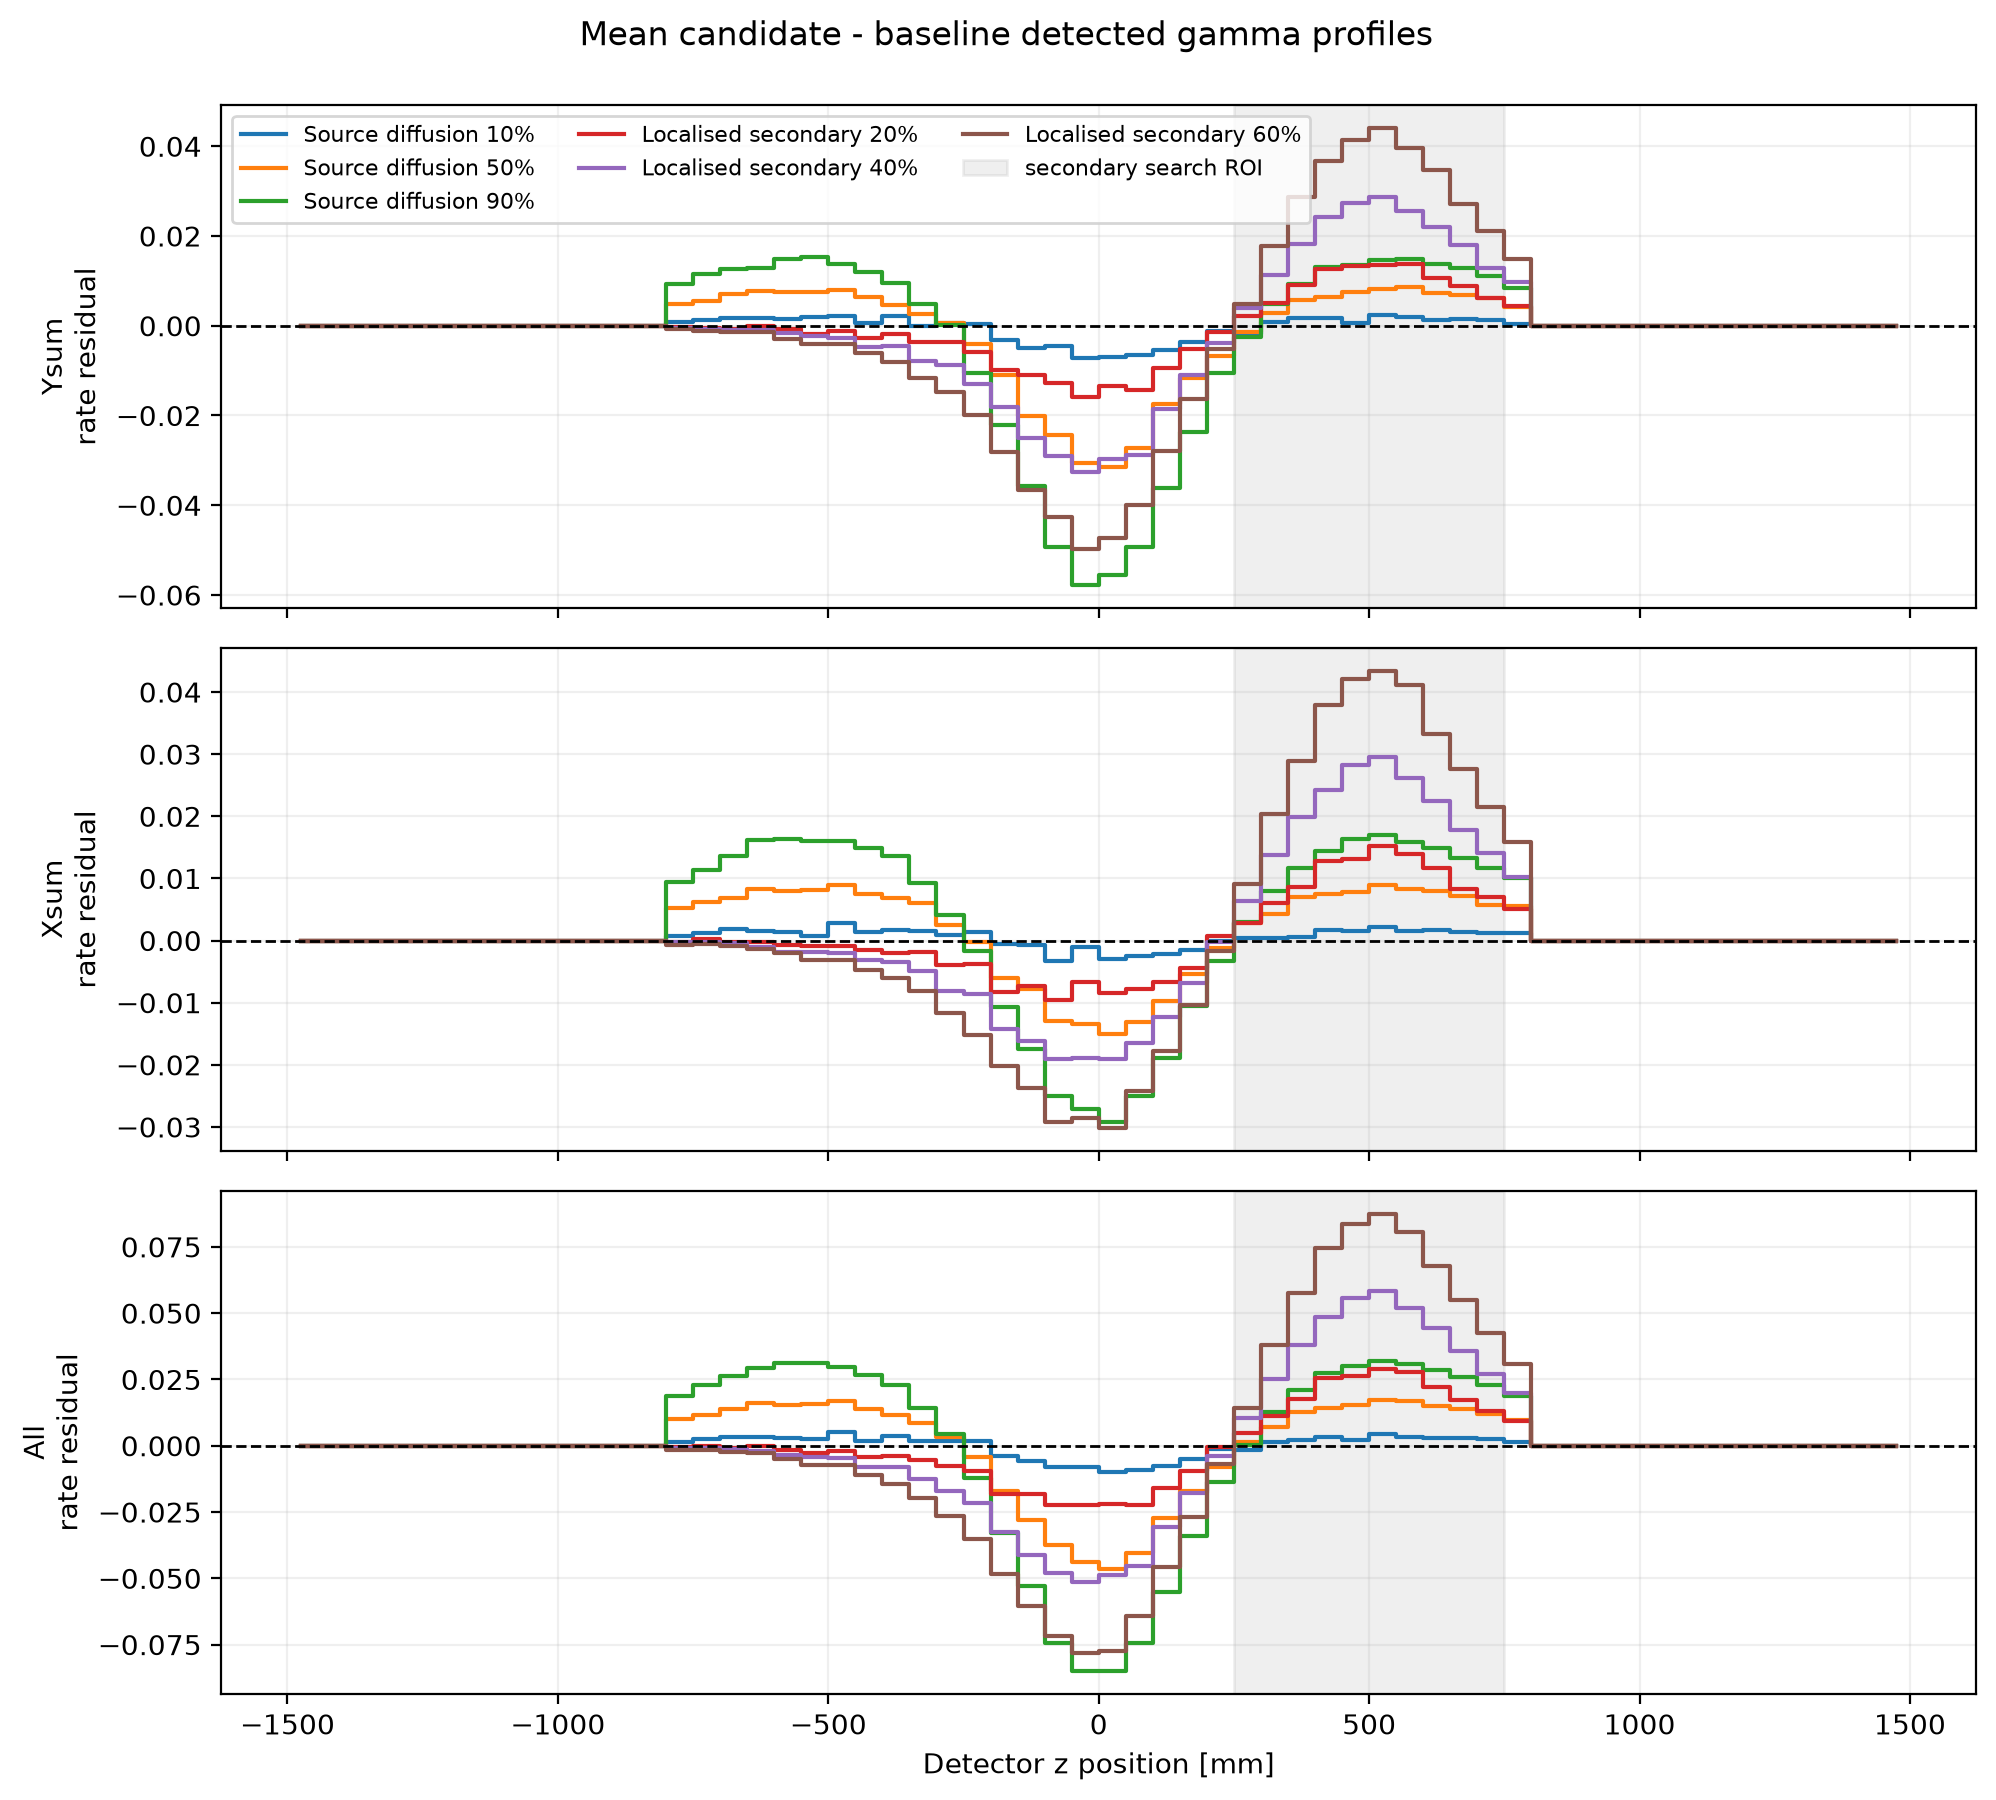
\includegraphics[width=\linewidth]{mean_residual_profiles_for_inference.png}
    \caption{\textit{Mean baseline-subtracted detector-hit profiles used as
    source-state features.}}
    \label{fig:residual_profiles}
\end{figure}

\subsection{Diffusion inference}

Residual-shape features were used to estimate the fraction of activity in
the broadly diffused component.  A regression trained on the retained and
broad-diffusion source states reconstructed diffusion fraction with
\(R^2=0.9987\) and a mean absolute error of about one percentage point.  The
high reconstruction accuracy in this controlled simulation reflects the
large change in spatial profile shape compared with the modest change in
total detector-entry rate.

\begin{figure}[!tbp]
    \centering
    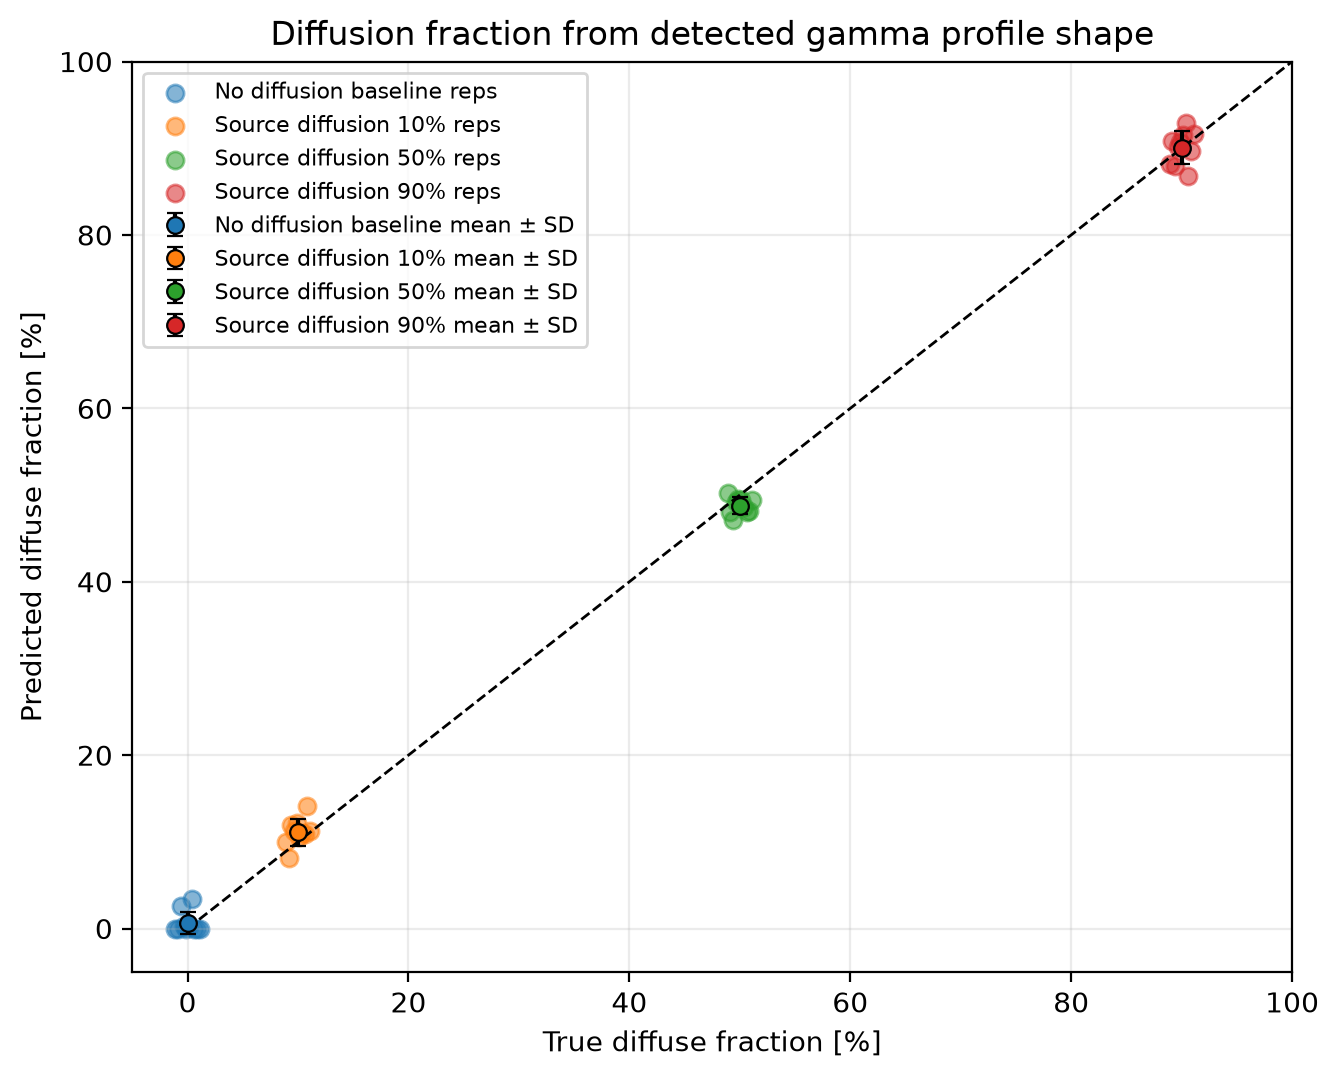
\includegraphics[width=0.85\linewidth]{diffusion_fraction_cv_prediction.png}
    \caption{\textit{Cross-validated diffusion-fraction prediction from
    residual profile features.}}
    \label{fig:diffusion_prediction}
\end{figure}

\subsection{Localised-source detection}

A displaced-region region-of-interest metric was used to test for activity
outside the expected retained-source region.  For localised cases, positive
residuals in the secondary-source region provided a source-position estimate.
The simulated localised source was centred at \(z=\SI{500}{mm}\).  Mean
reconstructed positions were approximately \(z=\SI{516}{mm}\),
\(\SI{528}{mm}\), and \(\SI{530}{mm}\) for 20\%, 40\%, and 60\% localised
activity, respectively.  Across the tested localised fractions, mean
position errors were \(16\)--\(\SI{30}{mm}\), with uncertainty decreasing
for larger localised fractions.

\begin{figure}[!tbp]
    \centering
    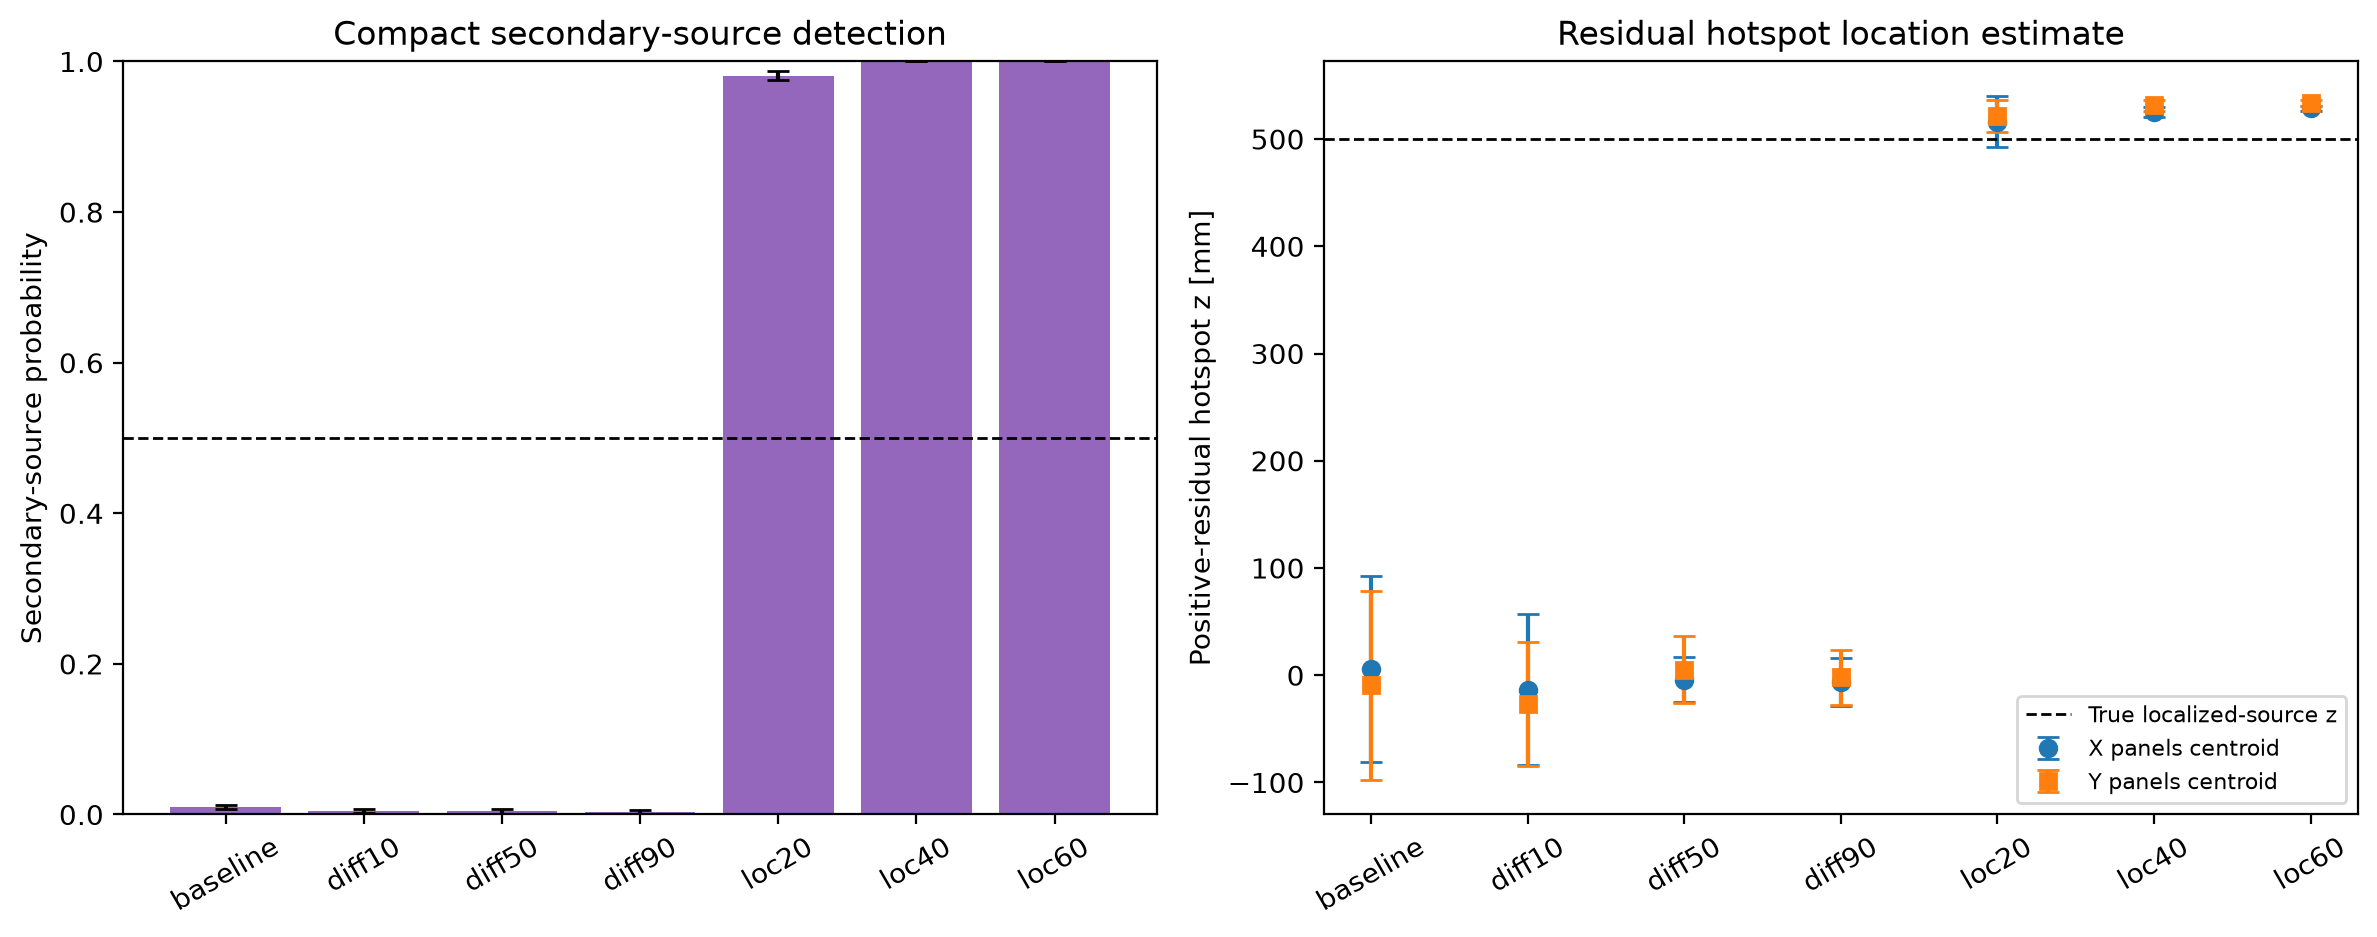
\includegraphics[width=\linewidth]{secondary_source_detection_and_location.png}
    \caption{\textit{Secondary-source detection and position summary from
    baseline-subtracted residuals.}}
    \label{fig:secondary_source}
\end{figure}

\subsection{Time-window detectability}

Detector hits were accumulated in increasing time windows and compared with
the retained-source baseline.  Detectability was defined using
candidate-baseline separation greater than \(3\sigma\) of the run-to-run
baseline variation.  In the 50-repetition analysis, 50--90\% broad diffusion
and 20--60\% localised displacement crossed threshold in about 1--2 hours,
while the 10\% broad-diffusion case required about 6 hours.  These results
suggest that the residual signal is not only present in integrated profiles,
but can emerge on treatment-relevant observation timescales in the simulated
geometry.

\section{Discussion}

The simulation shows that source localisation information is carried
primarily by spatial redistribution of decay-chain gamma hits.  This is
important because the total detector-entry rate changed by only a few
percent even for the largest broad-diffusion case.  A detector system relying
only on total count rate would therefore have limited ability to determine
whether activity remained in the applicator region or moved into the phantom.
By contrast, baseline-subtracted detector profiles separated retained,
diffused, and localised activity states in this idealised model.

The diffusion and localised-source metrics answer complementary questions.
The diffusion estimator quantifies broad redistribution using residual shape
features calibrated on diffuse source states.  The localised-source residual
tests for a compact off-applicator excess and estimates its longitudinal
position.  Reporting both quantities is preferable to interpreting any single
profile-width change as diffusion, because a compact displaced source can
also broaden or distort the observed profile.

Several limitations remain.  The detector panels in this study are idealised
hit counters, and the analysis does not yet include detector efficiency,
energy response, background, dead time, shielding, acquisition electronics,
or patient-specific anatomy.  The tested source states are simplified
sensitivity cases rather than biologically complete transport models.  Future
work should connect the activity-normalised residual profiles to measurable
count rates in a realistic detector and evaluate robustness under background
and clinical geometry assumptions.

\section{Conclusion}

Baseline-subtracted decay-chain gamma profiles distinguished retained,
broadly diffused, and locally displaced AlphaGlue activity in Geant4
simulations.  Diffusion fraction was estimated with \(R^2=0.9987\) and about
one percentage-point mean absolute error, while localised-source residuals
identified displaced activity with mean position errors of
\(16\)--\(\SI{30}{mm}\).  These findings support gamma-based post-treatment
monitoring as a route to assess source retention and redistribution after
targeted alpha therapy, provided future studies confirm the signal under
realistic detector-response and patient-scale conditions.

\section*{References}
{\small
\scriptsize
\begin{thebibliography}{1}
\bibitem{AlphaGlue2025}
L. Abu Sabah \textit{et al.}, ``AlphaGlue: A Novel Conceptual Delivery
Method for \(\alpha\) Therapy,'' \textit{BioMedInformatics} 5, 58, 2025.
\bibitem{laura}
L. Ballisat \textit{et al.}, ``Geant4 simulation of the enhanced in-vivo
\(^{220}\)Rn spread in DaRT,'' \textit{Phys. Med.} 135, 105005, 2025.
\bibitem{heger}
G. Heger \textit{et al.}, ``First measurements of radon-220 diffusion in
mice tumors,'' \textit{Med. Phys.} 51, 5045--5058, 2024.
\bibitem{Geant4}
S. Agostinelli \textit{et al.}, ``Geant4---a simulation toolkit,''
\textit{Nucl. Instrum. Methods Phys. Res. A} 506, 250--303, 2003.
\bibitem{dart}
L. Arazi \textit{et al.}, ``The treatment of solid tumors by alpha emitters
released from \(^{224}\)Ra-loaded sources,'' \textit{Phys. Med. Biol.} 55,
1203, 2010.
\bibitem{Geant4DNA}
S. Incerti \textit{et al.}, ``The Geant4-DNA project,''
\textit{Int. J. Model. Simul. Sci. Comput.} 1, 157--178, 2010.
\end{thebibliography}
}

\end{document}
